% !TEX ../report.tex

\section{Concepts fondamentaux de la suite \easypass{}}

\subsection{Présentation}
Le but d'\easypass{} est de proposer un password manager indépendant de tout serveur externe ou outil particulier. Les mots de passe sont stockés dans un fichier au format JSON. Pour garantir la sécurité, ce dernier est chiffré à l'aide d'un mot de passe selon l'algorithme AES-128-CBC tel qu'implémenté par l'outil opensource OpenSSL. Il est donc possible d'éditer ou récupérer ses mots de passe à l'aide d'une ligne de commande quelconque. \\
Les outils de la suite \easypass{} sont là pour offrir une couche \emph{user-friendly} à ce mécanisme de base. Ces outils se chargent de chiffrer/déchiffrer le fichier et d'en gérer le contenu (voir figure \ref{fig:schema-easypass}). 

Puisque nous ne faisons que manipuler un fichier, ce dernier peut être synchronisé ou sauvegardé avec de nombreux outils: Google Drive, Dropbox, etc. Sur Android, nous avons rendu l'utilisation de Dropbox obligatoire, mais ce n'est pas le cas sur les versions desktop.
Afin de rendre accessible le fichier depuis n'importe quel device, nous avons choisi de stocker le fichier sur Dropbox. 

\includeFigure{.8}{schema-easypass}{\easypass, architecture générale}

\subsection{Algorithme de chiffrement}

Le principe de \emph{password-based encryption} est de dériver une clé de chiffrement depuis un mot de passe fixe. La sécurité de cette méthode dépend alors de deux choses: a) la longueur du mot de passe, qui détermine également l'entropie de la clé générée, b) la PKDF (\emph{Password Key Derivation Function}), soit l'algorithme utilisé pour dériver une clé du mot de passe. Plus cette fonction prend du temps, plus une attaque brute-force deviendra difficile (manque de temps et de RAM).

\easypass{} utilise un chiffrement qui correspond aux lignes de commande OpenSSL suivante\footnote{AES est notamment utilisé par le gouvernement américain pour chiffrer ses données top secrètes. Ils utilisent cependant la variante 256-bits. Nous utilisons encore 128-bits pour rester compatible avec les autres outils de la suite (mise à jour prévue).}:

\begin{bashcode}
# encrypt
openssl enc -aes-128-cbc -salt -in file.json -out file.json.enc  

# decrypt
openssl enc -aes-128-cbc -d -a -in file.json.enc -out file.json 
\end{bashcode}


Pour mieux comprendre les mécanismes derrière le chiffrement AES-CBC ainsi que ses limites, nous recommandons notamment les ressources suivantes:

\begin{itemize}
    \item AES Encryption and Decryption with OpenSSL: \url{https://eclipsesource.com/blogs/2017/01/17/tutorial-aes-encryption-and-decryption-with-openssl/}
    \item Is password-based AES encryption secure at all? \url{https://crypto.stackexchange.com/questions/42538/is-password-based-aes-encryption-secure-at-all}
    \item Implémentation en Go du chiffrement \easypass{}: \url{https://github.com/derlin-easypass/easycmd-go/blob/master/crypto.go}
\end{itemize}

\section{Application Android}

fonctionnalités et captures aussi sur tablette !

Lors de la première utilisation d'application, l'utilisateur doit choisir son master password. Ce mot de passe servira à chiffrer le fichier de sauvegarde qui contiendra tous les mots de passe l'utilisateur.

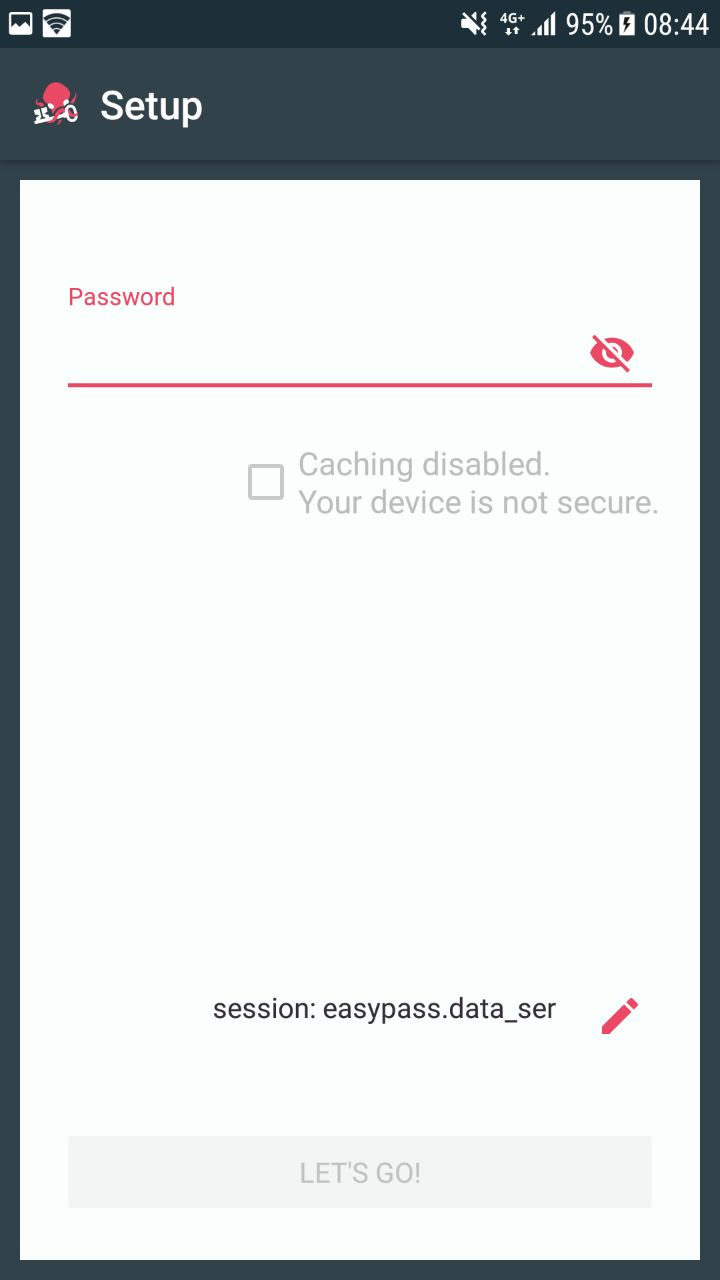
\includegraphics[height=10cm]{login.jpg}

L'utilisateur doit également autoriser l'accès de l'application à Dropbox.
L'application débute avec la vue login. Le master password est demandé afin de déchiffrer le fichier de sauvegarde des mots de passe. Ce mot de passe doit être compliqué afin de garantir la sécurité de l'application. Afin d'améliorer l'expérience utilisateur, l'application \easypass{} lui propose de le mettre en cache et d'utiliser les méthodes d'authifications fournies par Android.

L'application affiche le fichier utilisé pour sauvegarder les mots de passe. Il est possible de modifier le fichier selectionné.

La vue principale ou l'activité principale affiche la liste de tous les comptes de l'utilisateur. L'utilisateur peut ajouter un nouveau compte grâce au bouton flottant.

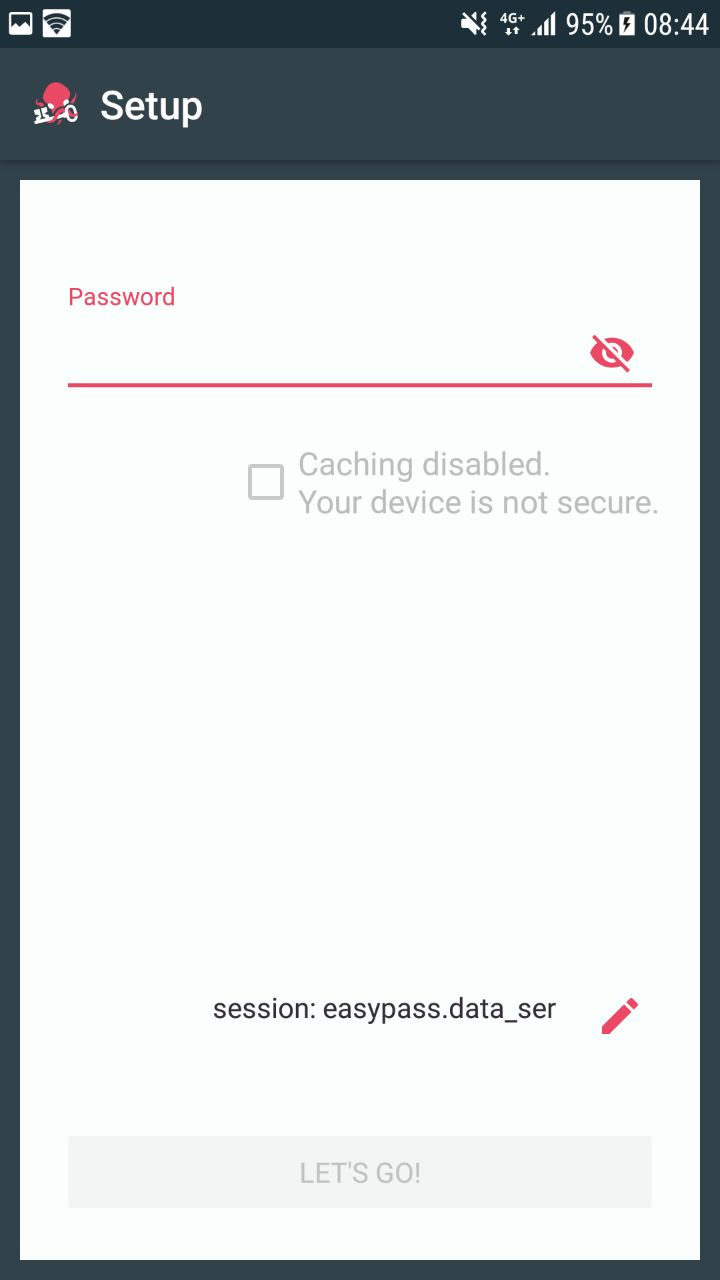
\includegraphics[height=10cm]{login.jpg}

Différentes informations peuvent être spécifiées pour le compte ainsi que le mot de passe. L'application \easypass{} propose également de générer un password aléatoire.

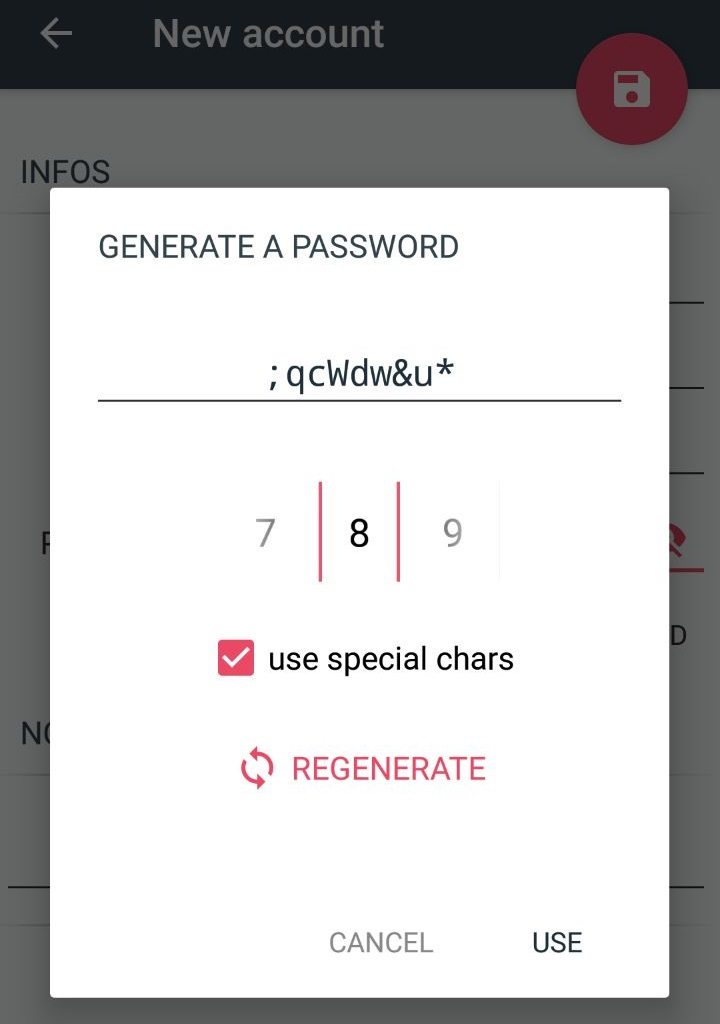
\includegraphics[height=7cm]{generate_password.jpg}

L'utilisateur peut générer un password aléatoire selon différents critères. La liste des caractères spéciaux utilisés peut être configurée dans les settings de l'application.

 L'objectif dans de l'application \easypass{} est de permettre à l'utilisateur de trouver le plus rapidement possible les informations du compte qu'il recherche. La liste affichée peut être triée par ordre et ordre inverse alphabetanumerique ou par date de création. Une fonction recherche est également proposé pour retrouver le nom du compte. Les comptes les plus utilisés peutvent être selectionnés par l'utilisateurs. Ils apparaitront en haut de la liste. 

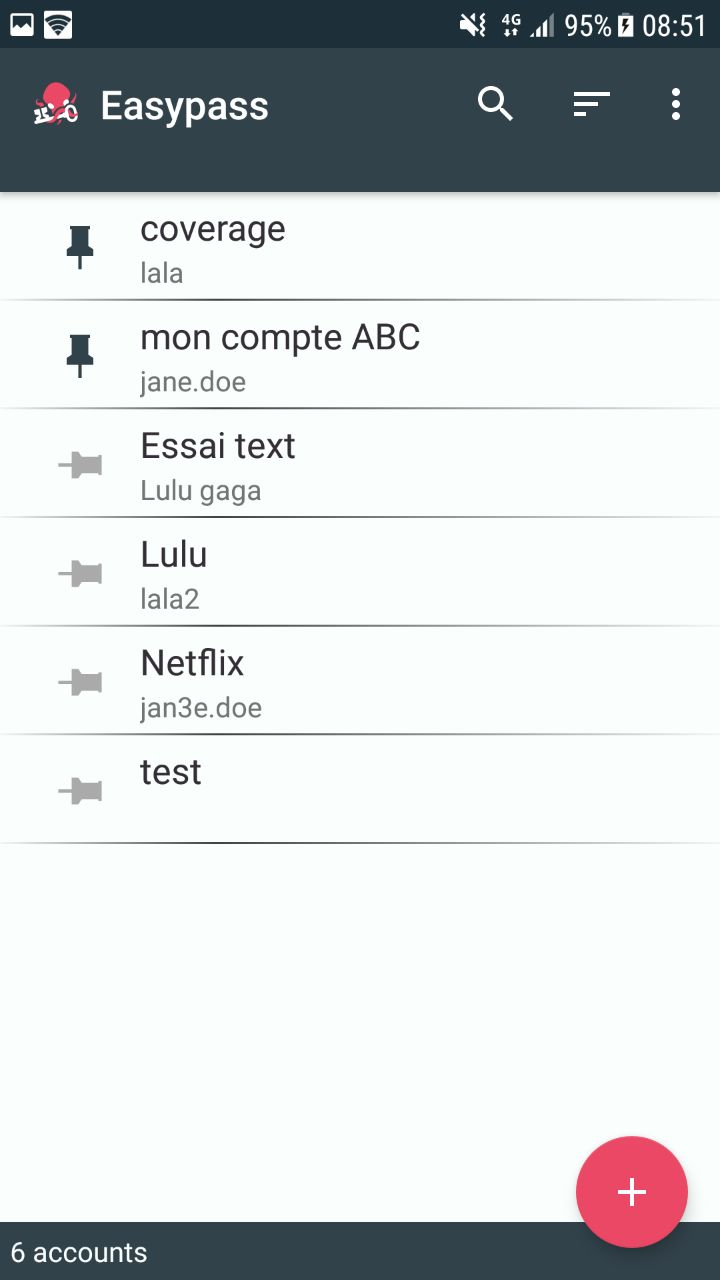
\includegraphics[height=10cm]{liste.jpg}

Lorsque l'utilisateur selectionne un compte, il peut voir dans le pannel toutes les opérations possible : 
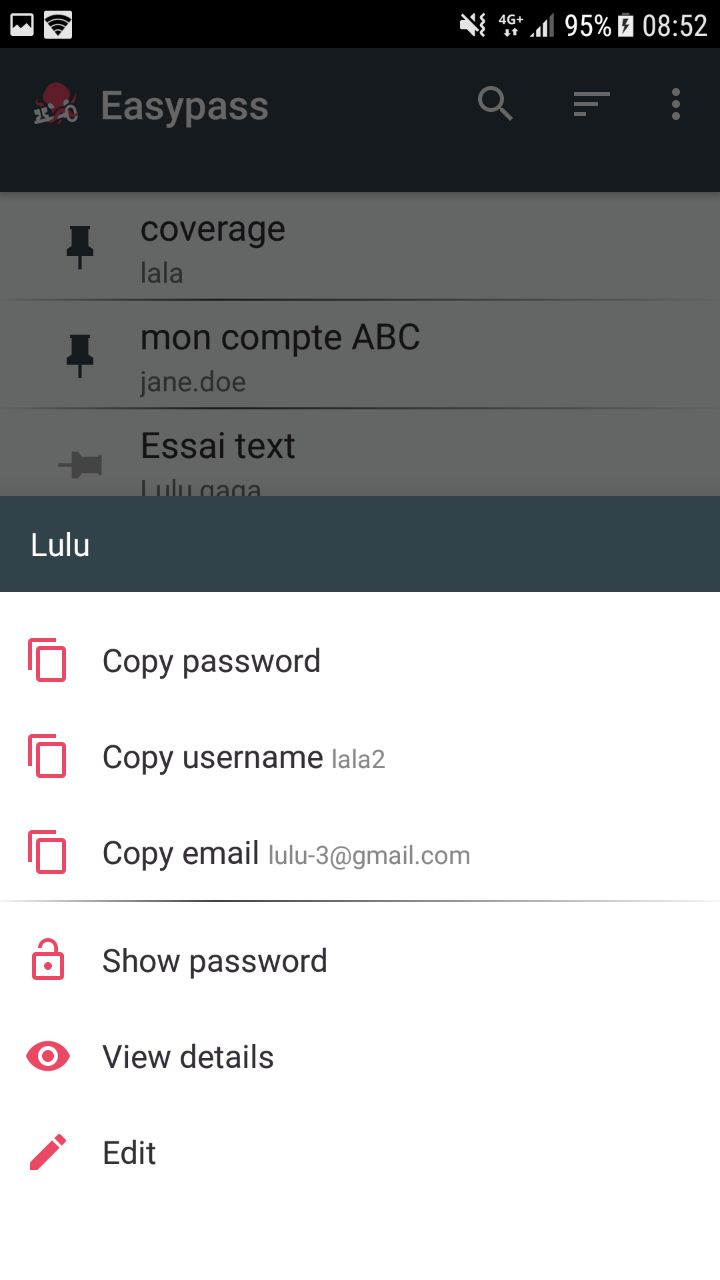
\includegraphics[height=10cm]{liste-edition.jpg}

Toujours dans un soucis d'améliorer l'expérieuce utilisateur, le pannel offre des raccourcis tel que copy email ou view password. Toutes les informations du compte sont disponibles dans la vue détail.

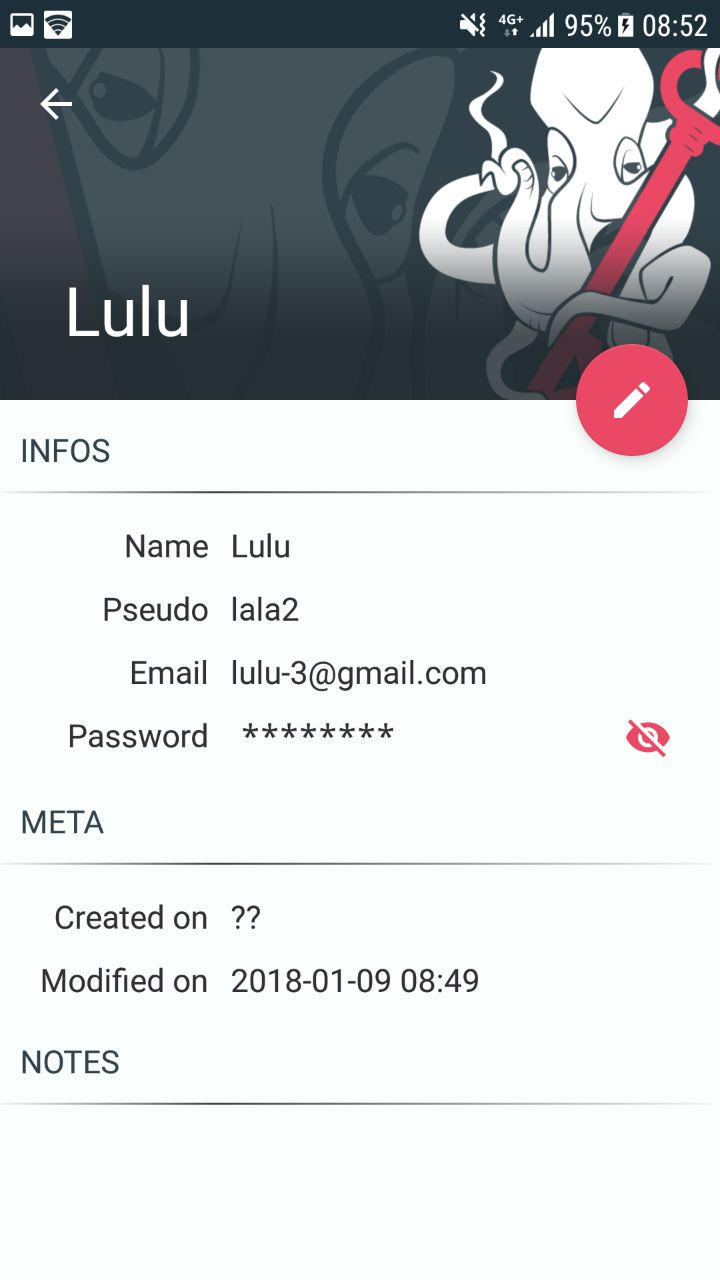
\includegraphics[height=10cm]{details.jpg}

Les options de configuration et personalisation sont disponible dans la vue settings atteignable depuis la vue principale. L'utilisateur peut ici configurer le master password et gérer le fichier synchroniser dans Dropbox.

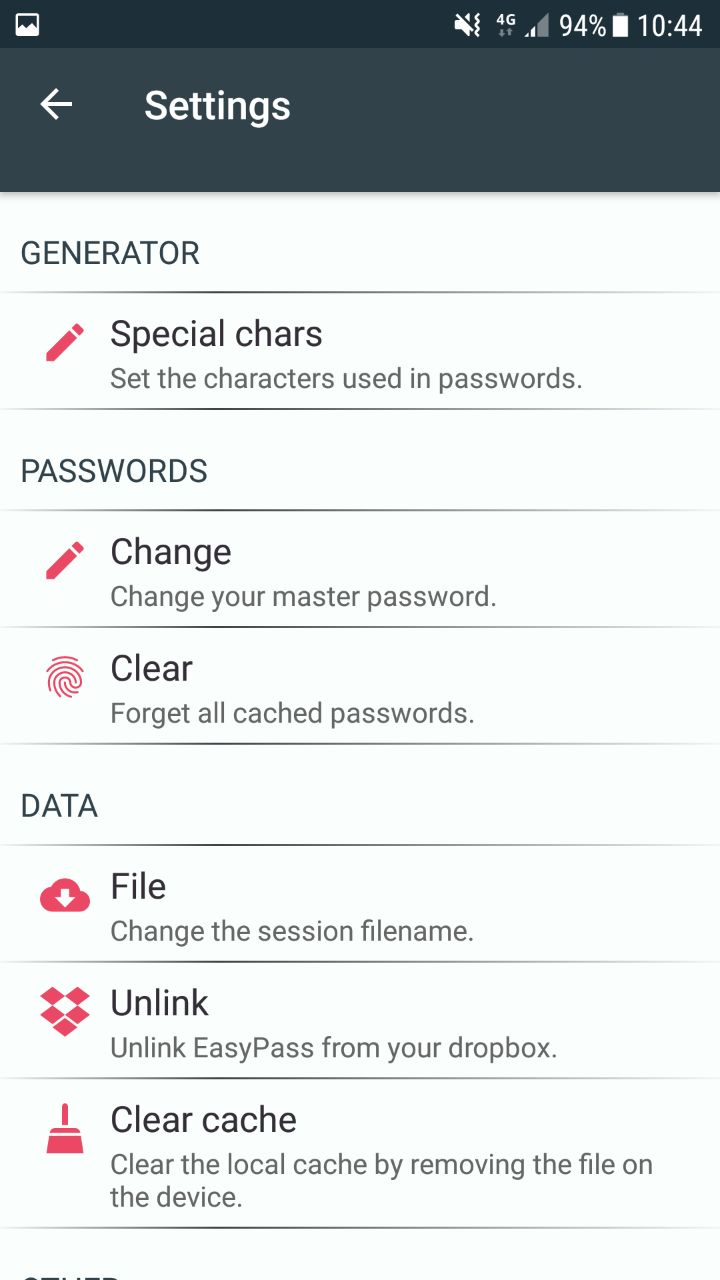
\includegraphics[height=10cm]{settings.jpg}

% exemple multiple images horizontal
\begin{center}
    \begin{minipage}{.3\textwidth}
        \includeFigure{1}{login}{Login 1}
    \end{minipage}
    \begin{minipage}{.3\textwidth}
        \includeFigure{1}{login}{Login 2}
    \end{minipage}
    \begin{minipage}{.3\textwidth}
        \includeFigure{1}{login}{Login 3}
    \end{minipage}        
\end{center}

% exemple de référence
blabla (see Figure \ref{fig:login}) blabla.

% exemple 1 figure
\includeFigure{.5}{generate_password}{caption text}